%\usepackage{graphicx}%! suppress = EquationReference
\chapter{Аналитический раздел}


В данном разделе будет проведен анализ предметной области, существующих решений и формулировка требований к разрабатываемой базе данных.

\section{Анализ предметной области}

Операции по техническому обслуживанию самолетов широко распространены внутри стран и между ними и выполняются как военными, так и гражданскими механиками.
Механики работают в аэропортах, на ремонтных базах, военных объектах.
Механиков нанимают пассажирские и грузовые перевозчики, подрядчики по техническому обслуживанию, сельскохозяйственные предприятия, а также владельцы государственного и частного флота.
Небольшие аэропорты могут обеспечить работой несколько механиков, в то время как в крупных узловых аэропортах и на базах технического обслуживания могут работать тысячи.
Работы по техническому обслуживанию делятся на те, которые необходимы для поддержания текущих повседневных операций (линейное техническое обслуживание), и на те, в процессе которых периодически проверяют, обслуживают и ремонтируют самолет (базовое техническое обслуживание).
Линейное техническое обслуживание включает в себя техническое обслуживание в пути (между посадкой и взлетом) и техническое обслуживание в ночное время.
Техническое обслуживание в пути состоит из эксплуатационных проверок и необходимого в полете ремонта для устранения несоответствий, обнаруженных во время полета.
Этот ремонт, как правило, незначителен, например, замена сигнальных ламп, шин и компонентов авионики, но может быть таким же масштабным, как замена двигателя.
Ночное техническое обслуживание более обширно и включает в себя любой ремонт, отложенный во время дневных полетов.

Сроки, распределение работников и характер технического обслуживания самолетов контролируются каждой авиакомпанией и документируются в ее руководстве по техническому обслуживанию.
Эти плановые мероприятия по техническому обслуживанию обеспечивают проверку, техническое обслуживание и ремонт всего воздушного судна через соответствующие промежутки времени.
Проверки технического обслуживания более низкого уровня могут быть включены в работы по техническому обслуживанию линии, но более обширные работы выполняются на базе технического обслуживания.
Повреждения самолета и отказы компонентов устраняются по мере необходимости~\cite{otplane}.

Время оборота самолета (\textit{англ.} TAT --- turnaround time) --- это общее время, которое требуется для выполнения всех необходимых действий для подготовки самолета к следующему рейсу.
Из--за ограниченного пространства вокруг самолета, операции оборота должны выполняться в точной хронологической последовательности: некоторые из них обязательно должны выполняться последовательно, в то время как другие могут выполняться одновременно.
Эффективность оборота самолета можно определить как способность выполнения необходимых операций в доступное время для обеспечения пунктуального вылета.

Наземное обслуживание самолета --- это сервисный процесс с жесткими требованиями, включающий более 10 взаимосвязанных подпроцессов и вовлекающий более 30 различных сотрудников.

На рисунке~\ref{fig:tat} представлена схема процесса наземного обслуживания самолета, включающая три основные категории обслуживания: пассажиров, багажа и груза, а также самого самолета.

\begin{figure}[h]
    \centering
    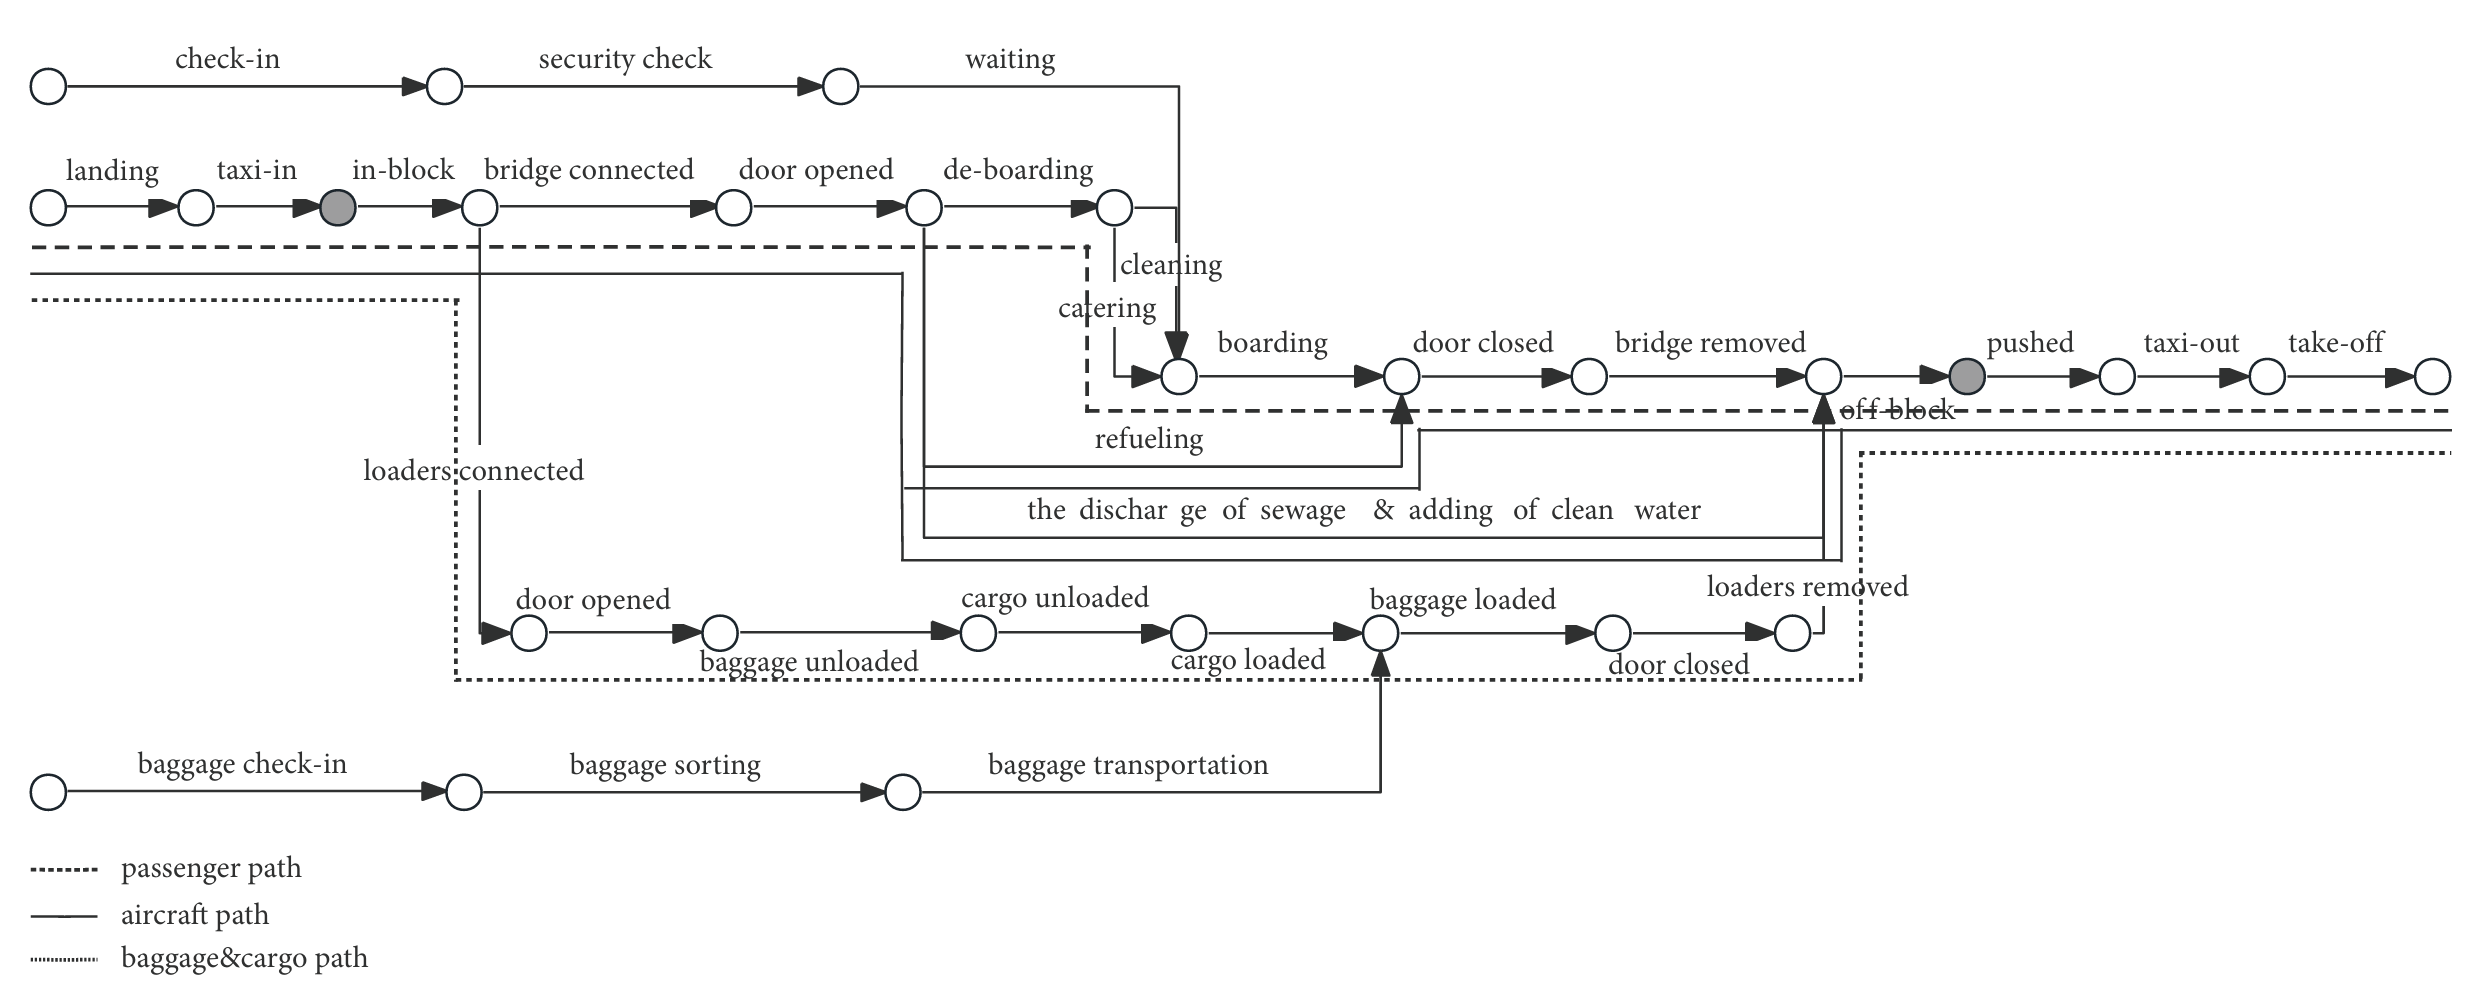
\includegraphics[scale=0.25]{inc/tat}
    \caption{Схема процессов наземного обслуживания самолета}
    \label{fig:tat}
\end{figure}

Пассажиры проходят регистрацию, проверку безопасности и ожидают посадки.
После посадки самолета пассажиры выходят через подключенный мост и проходят высадку.
После уборки и обслуживания питания начинается посадка пассажиров на следующий рейс.

Багаж регистрируется, сортируется и транспортируется к самолету.
После посадки самолета багаж выгружается и новый багаж загружается.
После завершения загрузки багажных отсеков двери закрываются.

Самолет проходит этапы от посадки до взлета, включая такси, подключение моста, открытие дверей, разгрузку и загрузку багажа и груза, заправку, уборку, обслуживание питания и техническое обслуживание.
После завершения всех операций, мост убирается, самолет выталкивается, проходит такси и взлетает.


Эта схема иллюстрирует важность координации и последовательности действий для обеспечения эффективного и своевременного оборота самолета~\cite{trt-timeestimation}.


\section{Анализ существующих решений}

Существует несколько решений в сфере мониторинга полетов, которые обеспечивают отслеживание воздушного движения в реальном времени:
\begin{enumerate}[label=\arabic*)]
    \item Flightradar24 --- это глобальный сервис отслеживания рейсов, который предоставляет информацию о 1000 воздушных судов по всему миру в режиме реального времени~\cite{flightradar24};
    \begin{figure}[h]
        \centering
        \includegraphics[scale=0.1]{inc/flightradar24}
        \caption{Пример отслеживания полетов на Flightradar24}
        \label{fig:flightradar24}
    \end{figure}
    \item FlightAware --- это цифровая авиационная компания, которая управляет крупнейшей в мире платформой отслеживания полетов и сбора данных.
    Благодаря глобальной связи с каждым сегментом авиации, FlightAware предоставляет более 10000 эксплуатантам воздушных судов и поставщикам услуг, а также более 13000 000 пассажиров глобальные решения для отслеживания полетов, технологии прогнозирования, аналитики и инструменты принятия решений~\cite{flightaware}.
    \begin{figure}[h]
        \centering
        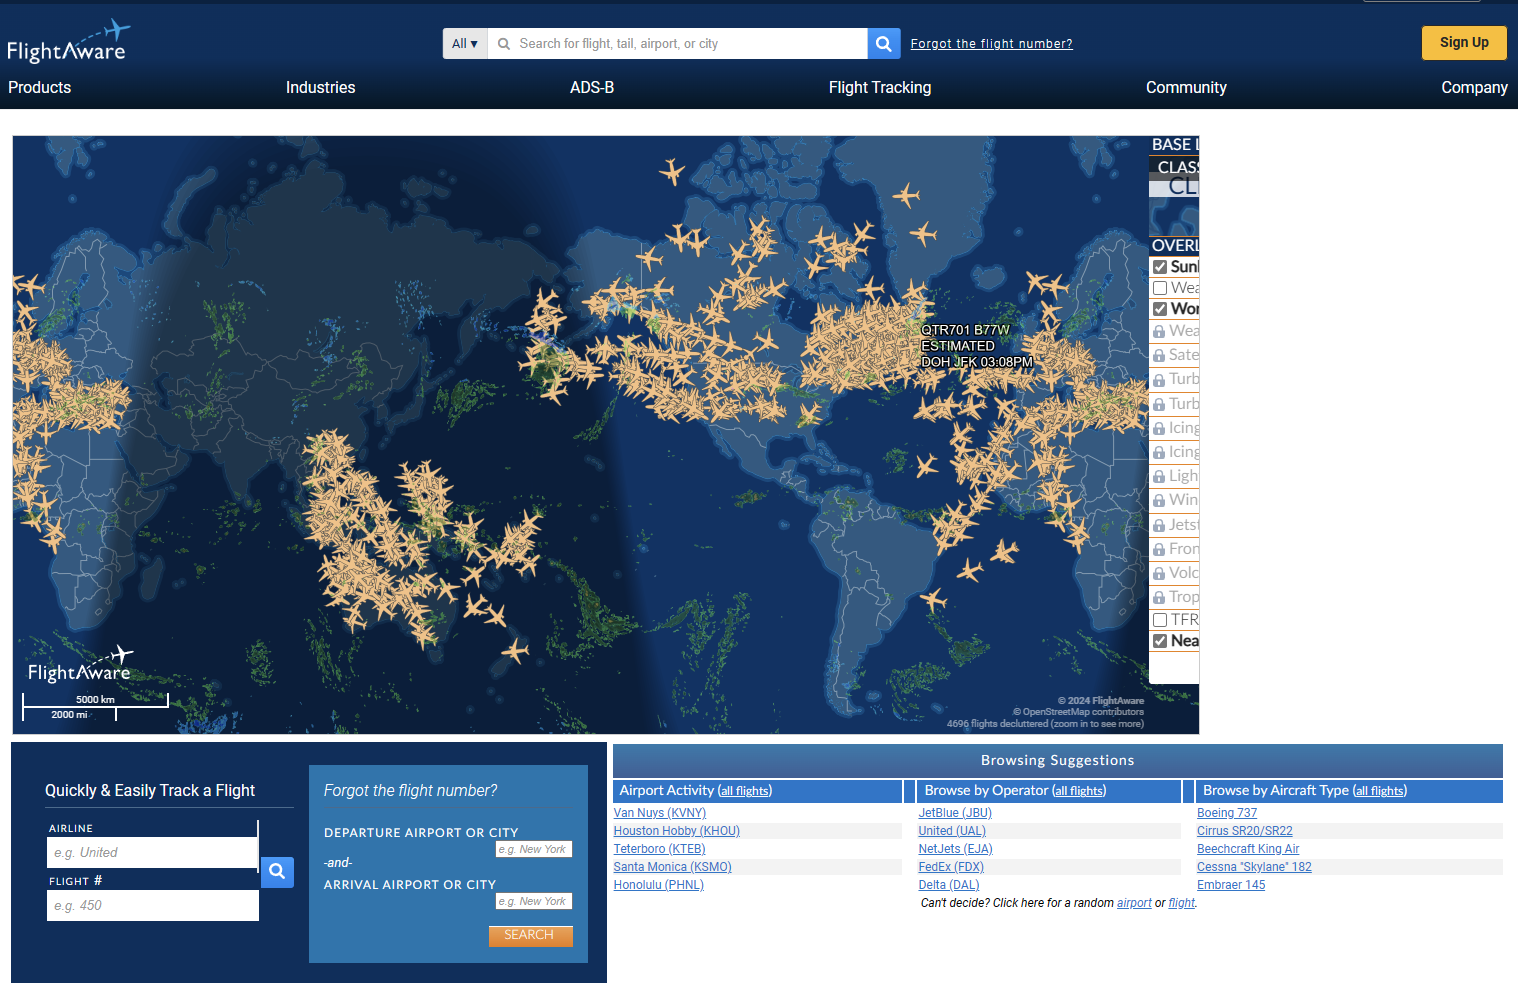
\includegraphics[scale=0.3]{inc/flightaware}
        \caption{Пример отслеживания полетов на FlightAware}
        \label{fig:flightaware}
    \end{figure}
\end{enumerate}



%\section{Формулировка требований к \newline разрабатываемой базе данных}
%
%В рамках поставленной цели необходимо разработать базу данных, которая будет хранить информацию о полетах, аэропортах, самолетах и экипажа самолета, а также API для доступа к данным и последующей возможности создания веб--приложения об прогнозировании вероятности задержки рейса.
%
%API должно обеспечивать доступ ко всем сущностям базы данных.
%Должна быть предусмотрена функциональность для добавления, удаления или изменения каждой из сущностей.
%Также должна быть возможность получения информации о полетах, аэропортах, самолетах и экипажа самолёта.
%

\section{Формализация информации, хранимой в базе данных}

Для наполнения данными базы данных были использованы датасеты с платформы Kaggle, что позволило провести более глубокий анализ полученных результатов.
Это платформа для машинного обучения и аналитики данных, которая предоставляет доступ к множеству датасетов, подготовленных сообществом~\cite{kaggle}.
На платформе Kaggle были найдены датасеты, содержащие информацию о задержках рейсов, аэропортах, авиакомпаниях и полетах.

После анализа датасетов были выделены следующие сущности:
\begin{enumerate}[label=\arabic*)]
    \item полет;
    \item задержка;
    \item аэропорт;
    \item авиакомпания;
    \item самолет;
    \item экипаж;
    \item отчет;
    \item система.
\end{enumerate}

На рисунке~\ref{fig:er} представлена ER--диаграмма сущностей системы в нотации Чена.

\begin{figure}[H]
    \centering
    \includegraphics[scale=0.45]{inc/Drawing1}
    \caption{ER -- диаграмма для базы данных}
    \label{fig:er}
\end{figure}

\section{Система ролей в базе данных}

Ролевая модель в базе данных состоит из трех ролей:
\begin{enumerate}[label=\arabic*)]
    \item гость --- пользователь, у которого есть доступ к чтению сущностей полета, аэропорта, авиакомпании, задержки, а также возможность получить информацию о вероятности задержки конкретного перелета;
    \begin{figure}[H]
        \centering
        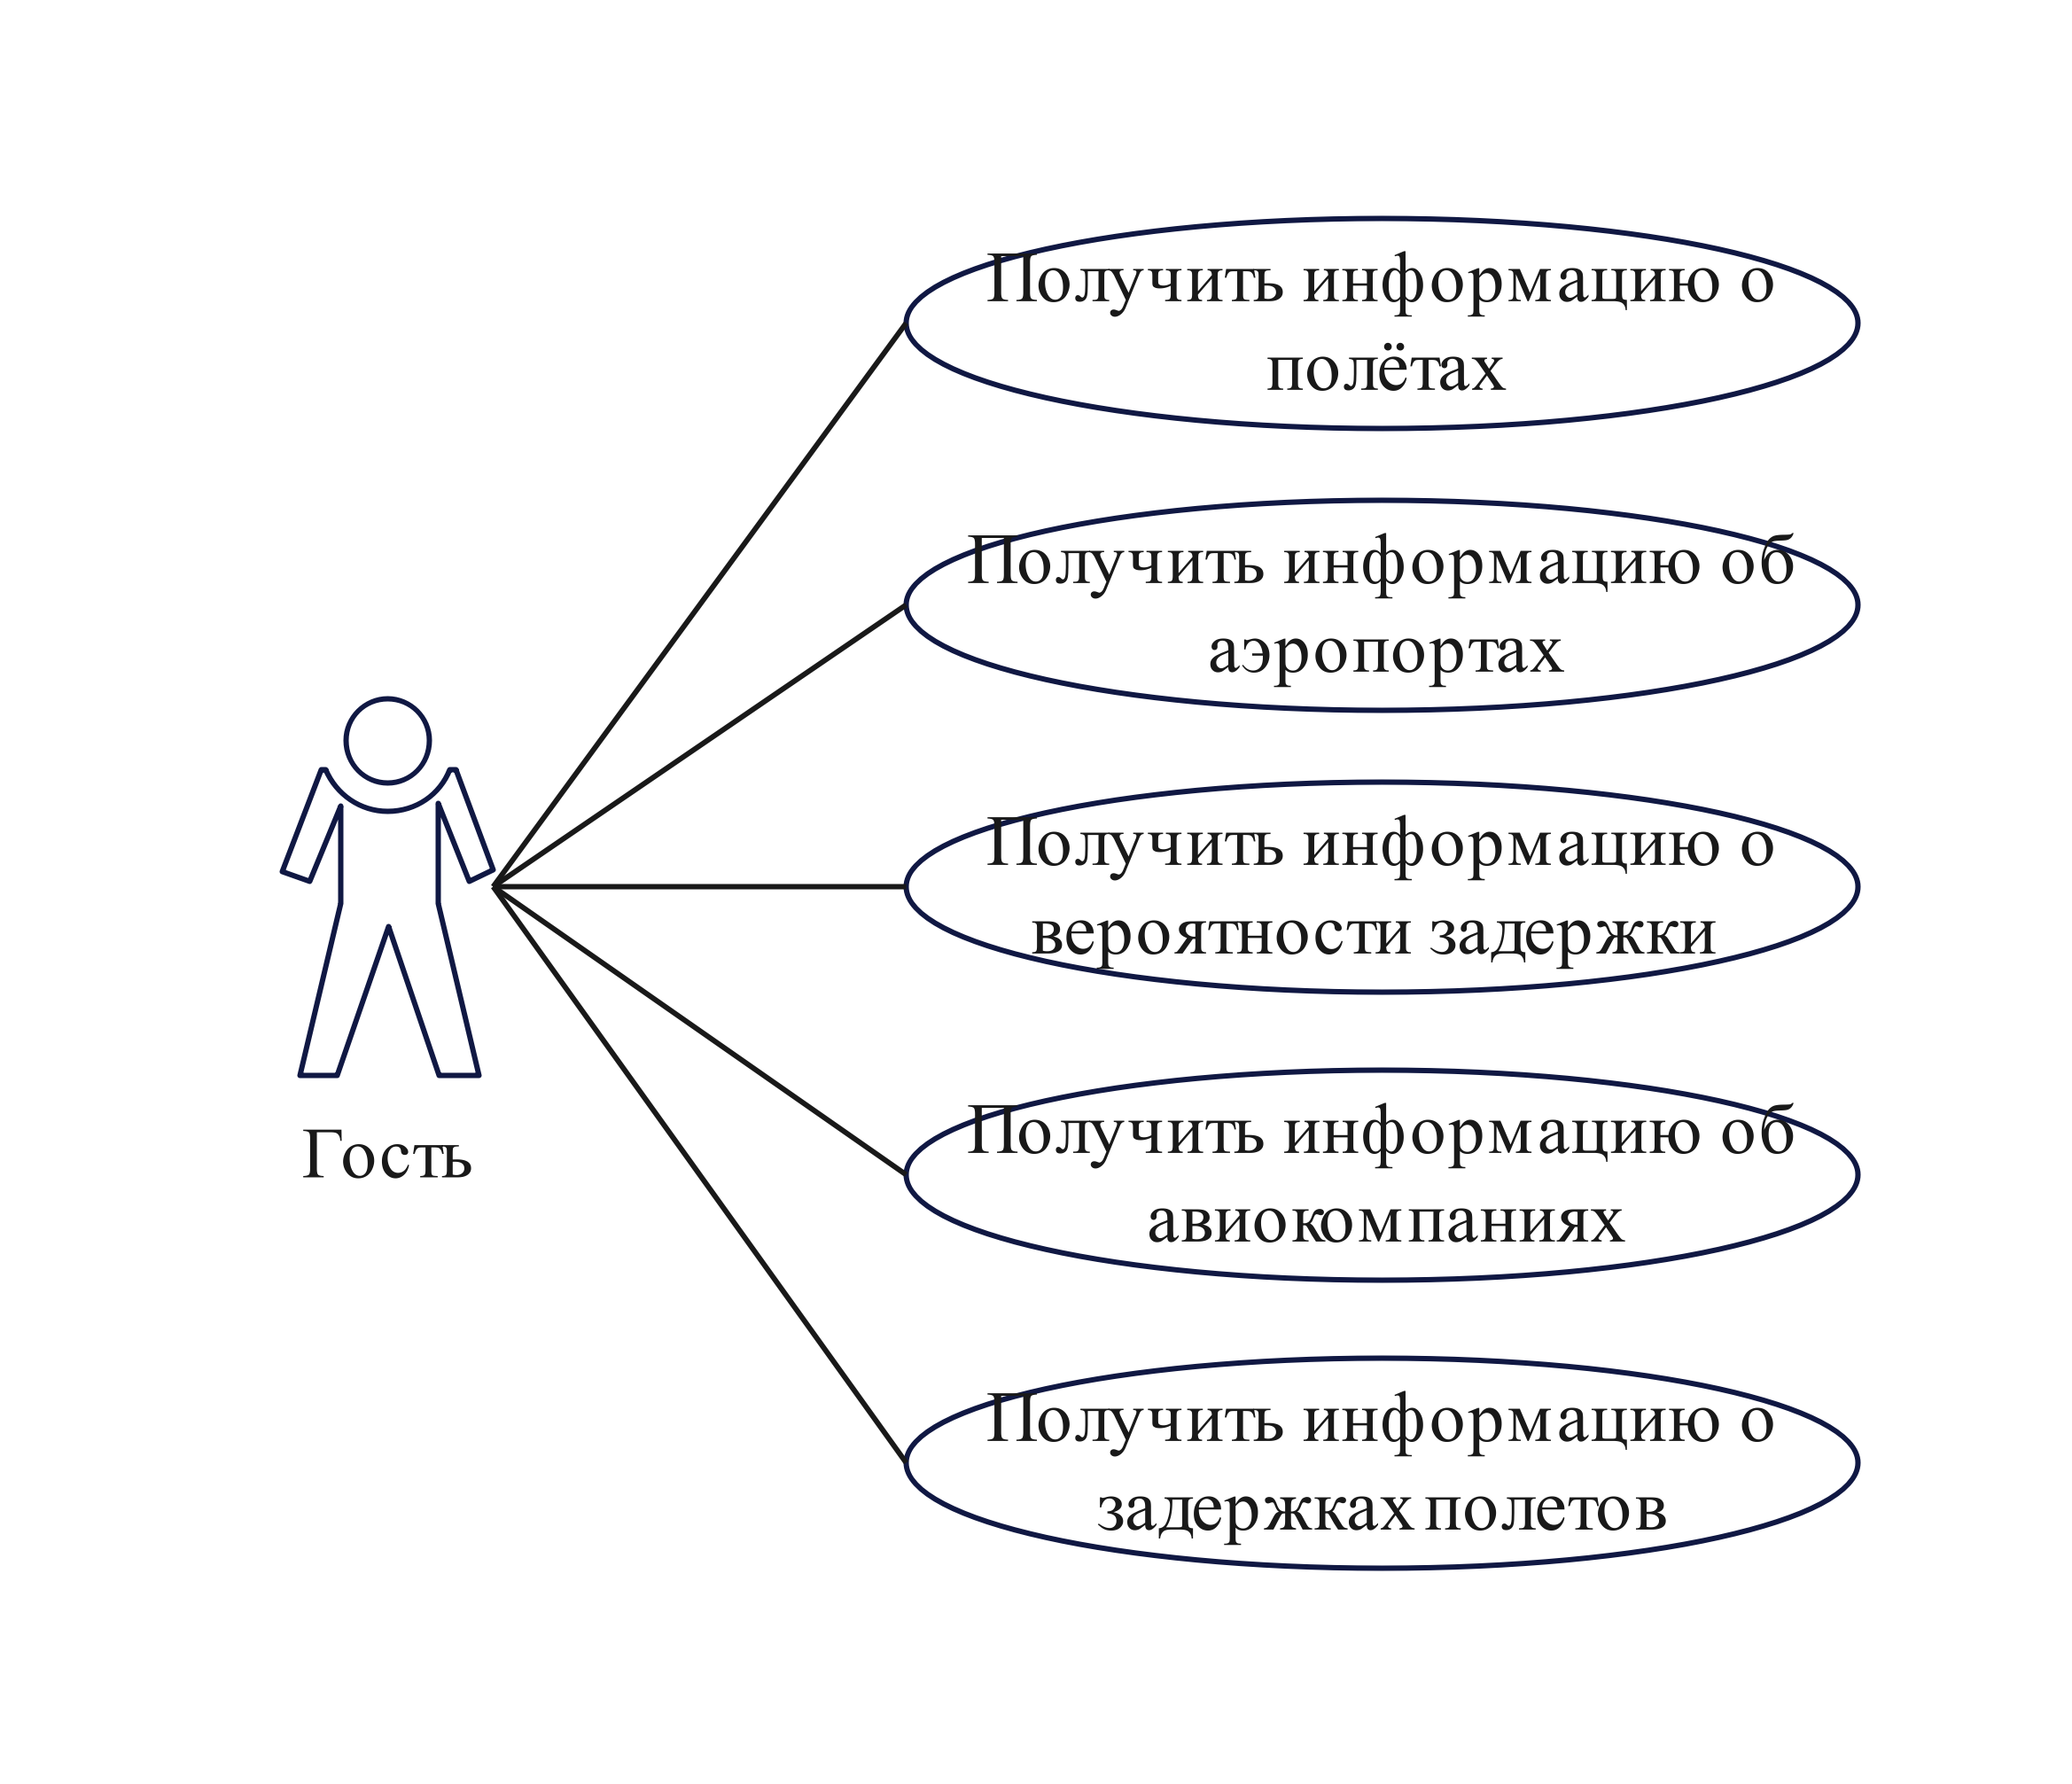
\includegraphics[scale=0.7]{inc/Guest_role}
        \caption{Use--case диаграмма для роли "гость"}
        \label{fig:guest_role}
    \end{figure}

    \item сотрудник --- пользователь, который имеет доступ к чтению и записи сущностей отчета и системы;
    \begin{figure}[H]
        \centering
        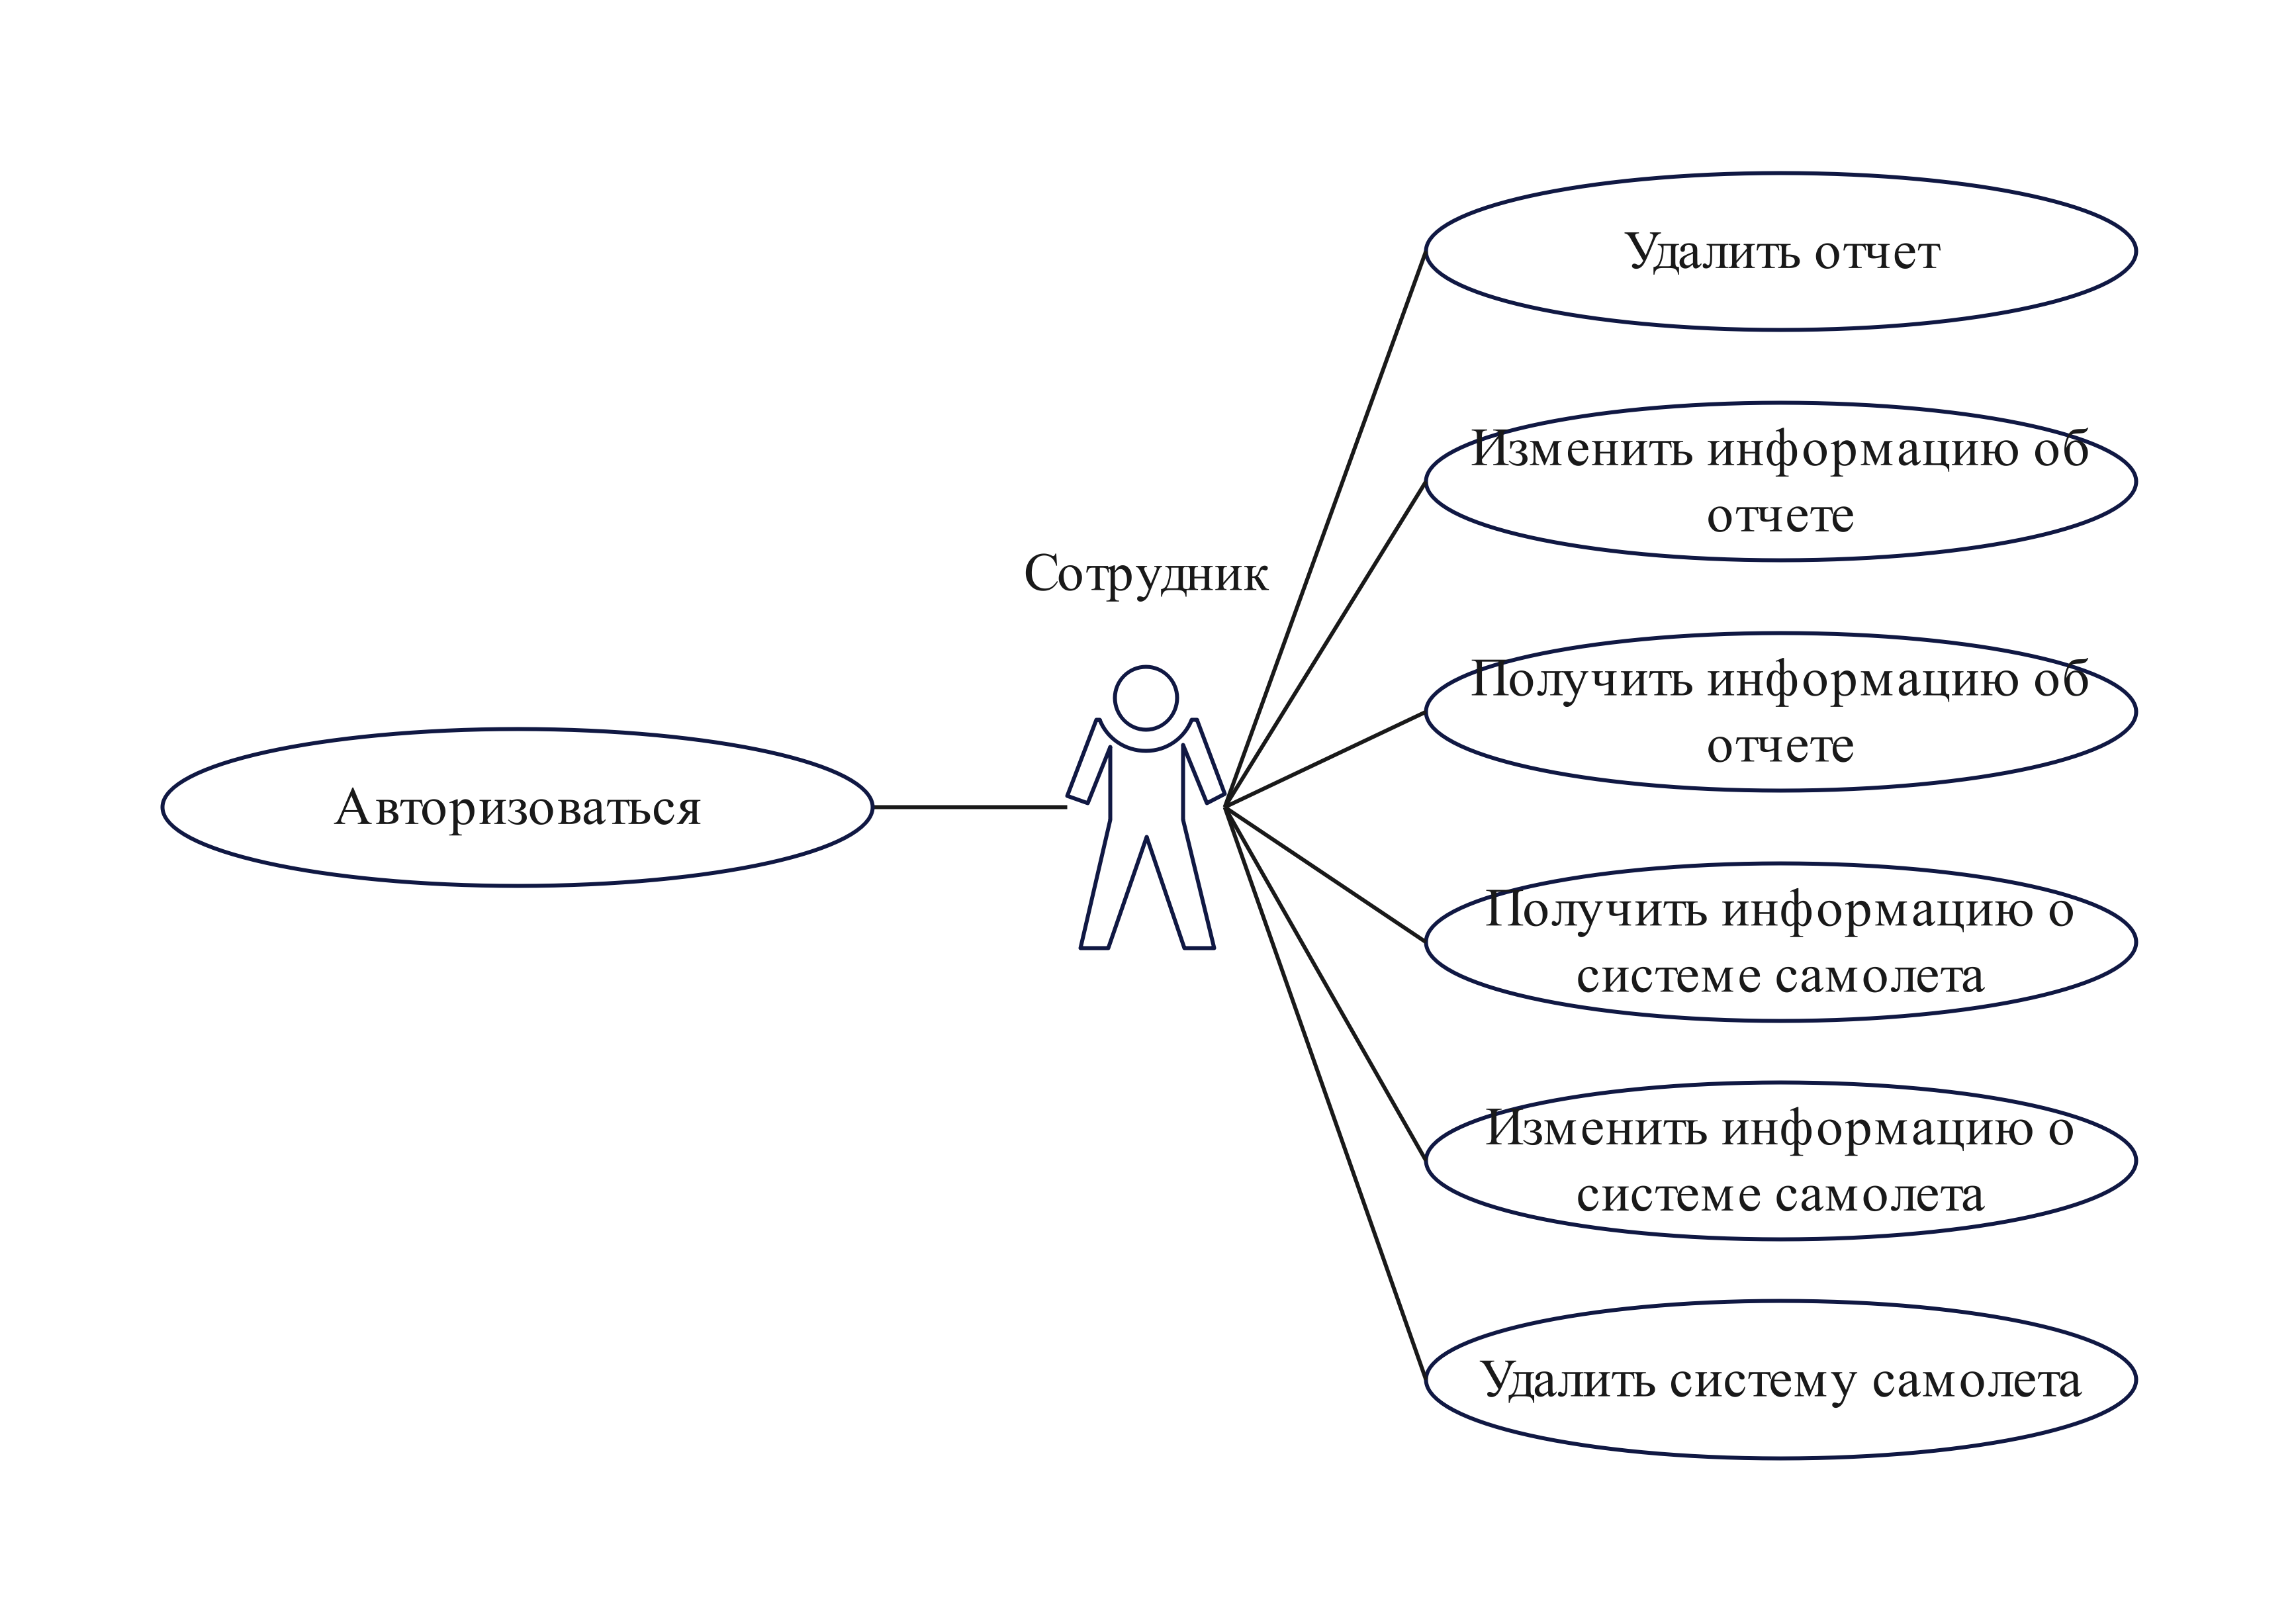
\includegraphics[scale=0.7]{inc/Employee_role}
        \caption{Use--case диаграмма для роли "сотрудник"}
        \label{fig:client_role}
    \end{figure}

    \item администратор --- пользователь, имеющий полный контроль над всеми сущностями, а также возможность получить информацию о вероятности задержки конкретного перелета.
    \begin{figure}[H]
        \centering
        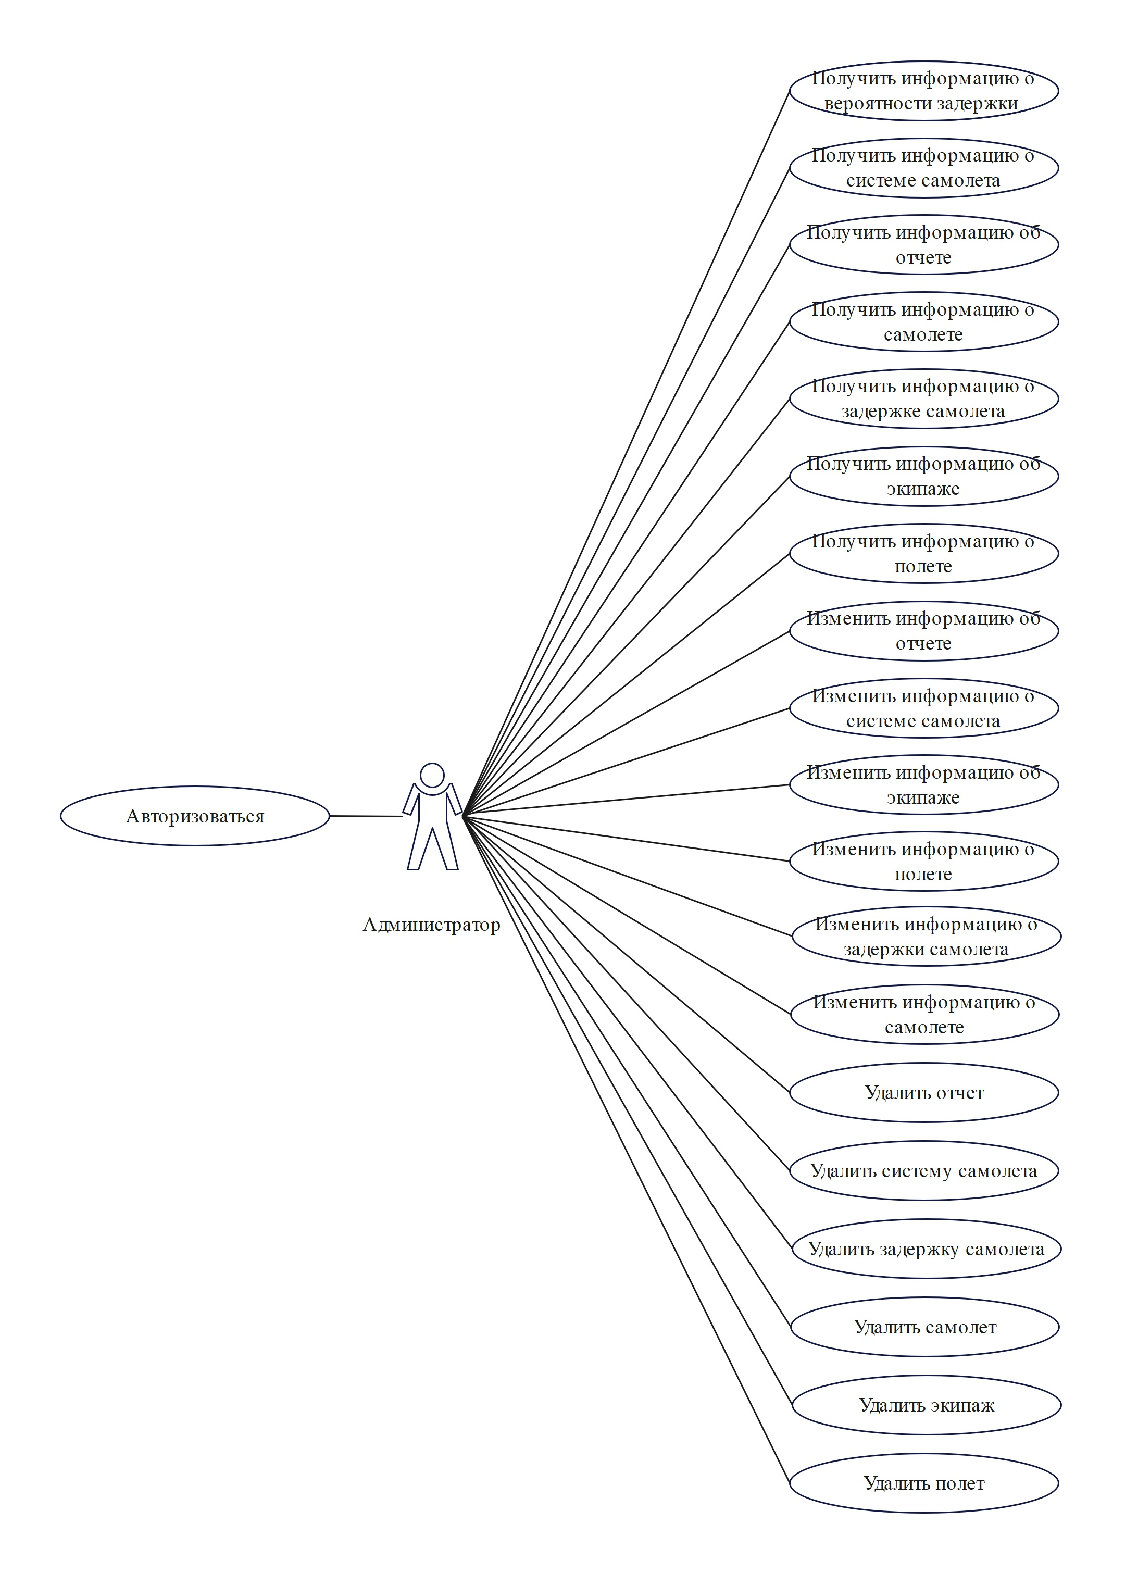
\includegraphics[scale=0.7]{inc/Admin_role}
        \caption{Use--case диаграмма для роли "администратор"}
        \label{fig:admin_role}
    \end{figure}
\end{enumerate}
\newpage


\section{Выбор модели базы данных}
По модели хранения данных выделяют следующие СУБД \newline(\textit{англ.} DBMS --- database management system):

\begin{enumerate}[label=\arabic*)]
    \item дореляционные;
    \item реляционные;
    \item постреляционные.
\end{enumerate}

Ниже рассмотрены основные модели баз данных.

\subsection{Дореляционные СУБД}
\begin{enumerate}[label=\arabic*.]
    \item Инвертированные списки --- БД на основе инвертированных списков представляет собой совокупность файлов, содержащих записи (таблиц).
    Для записей в файле определен некоторый порядок, диктуемый физической организацией данных.
    Для каждого файла может быть определено произвольное число других упорядочений на основании значений некоторых полей записей (инвертированных списков).
    Обычно для этого используются индексы.
    В такой модели данных отсутствуют ограничения целостности как таковые.
    Все ограничения на возможные экземпляры БД задаются теми программами, которые работают с БД.
    Одно из немногих ограничений, которое все-таки может присутствовать - это ограничение, задаваемое уникальным индексом~\cite{lekcii}.
    \item Иерархическая модель данных --- иерархическая модель БД состоит из объектов с указателями от родительских объектов к потомкам, соединяя вместе связанную информацию.
    Иерархические БД могут быть представлены в виде дерева~\cite{lekcii}.
    \item Сетевая модель данных --- к основным понятиям сетевой модели БД относятся: элемент (узел), связь.
    Узел — это совокупность атрибутов данных, описывающих некоторый объект.
    Сетевые БД могут быть представлены в виде графа.
    В сетевой БД логика процедуры выборки данных зависит от физической организации этих данных.
    Поэтому эта модель не является полностью независимой от приложения.
    Другими словами, если необходимо изменить структуру данных, то нужно изменить и приложение~\cite{lekcii}.

    На рисунке~\ref{fig:network-model} представлена сетевая модель данных.

    \begin{figure}[h]
        \begin{center}
            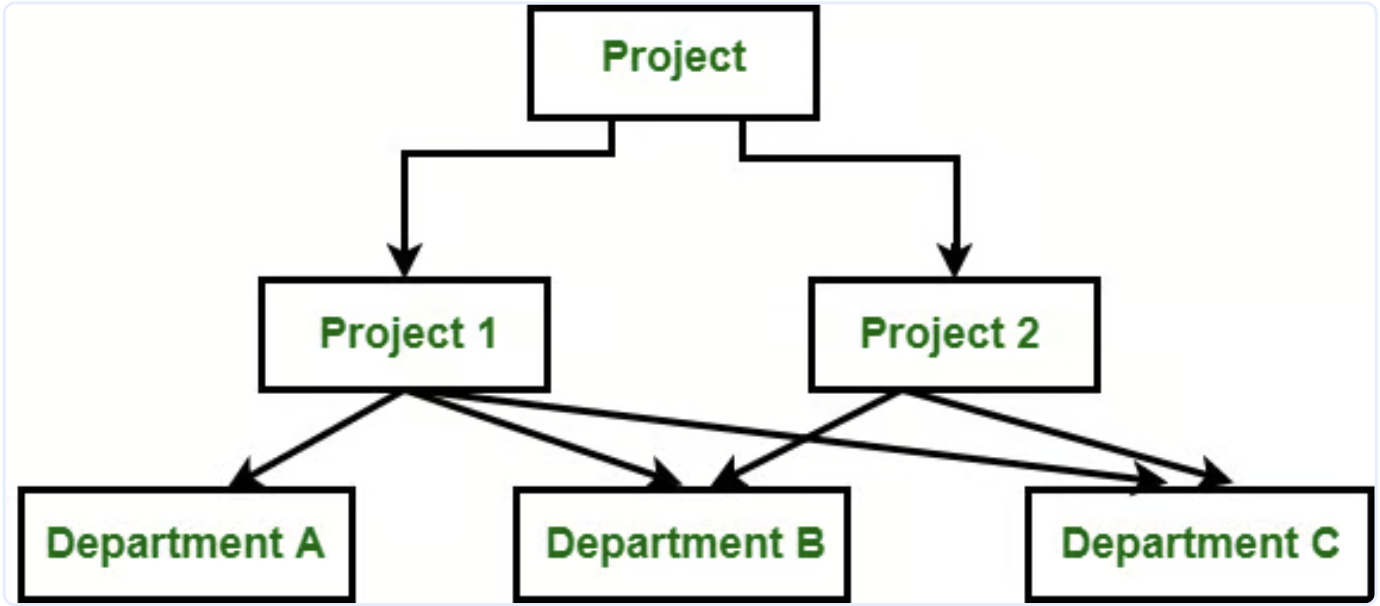
\includegraphics[scale=0.3]{inc/network-model}
            \caption{Сетевая модель данных}
            \label{fig:network-model}
        \end{center}
    \end{figure}
\end{enumerate}

\subsection{Реляционная модель данных}
Реляционная модель данных включает в себя следующие аспекты:

\begin{enumerate}[label=\arabic*)]
    \item структурный аспект --- данные в базе данных представлены в виде набора отношений, также известных как таблицы.
    \item целостностный аспект --- отношения (таблицы) должны соответствовать определенным условиям целостности, гарантирующим правильное и надежное хранение данных.
    \item манипуляционный аспект --- манипулирование данными в отношениях осуществляется с помощью средств реляционной алгебры и/или реляционного исчисления.
    Это позволяет выполнять различные операции над данными, такие как выборка, вставка, обновление и удаление.
    Кроме того, реляционная модель данных включает в себя теорию нормализации, которая помогает улучшить организацию данных в базе данных и избежать избыточности и аномалий.
    В 1985 году доктор Кодд сформулировал двенадцать правил, которым должна соответствовать настоящая реляционная база данных.
    Эти правила являются полуофициальным определением понятия реляционной базы данных и предоставляют стандарт для оценки соответствия реляционной базы данных этой модели~\cite{lekcii}.
\end{enumerate}


\section*{Выводы}
В данном разделе проанализированы техническое обслуживание самолетов, процесс оборота самолета и наземное обслуживание.
Определены требования к разрабатываемой базе данных, выделены основные сущности для хранения данных.
Разработана система ролей для пользователей на уровне базы данных.
Выбрана реляционная модель данных для реализации базы данных.